\documentclass[main.tex]{subfiles}

\begin{document}

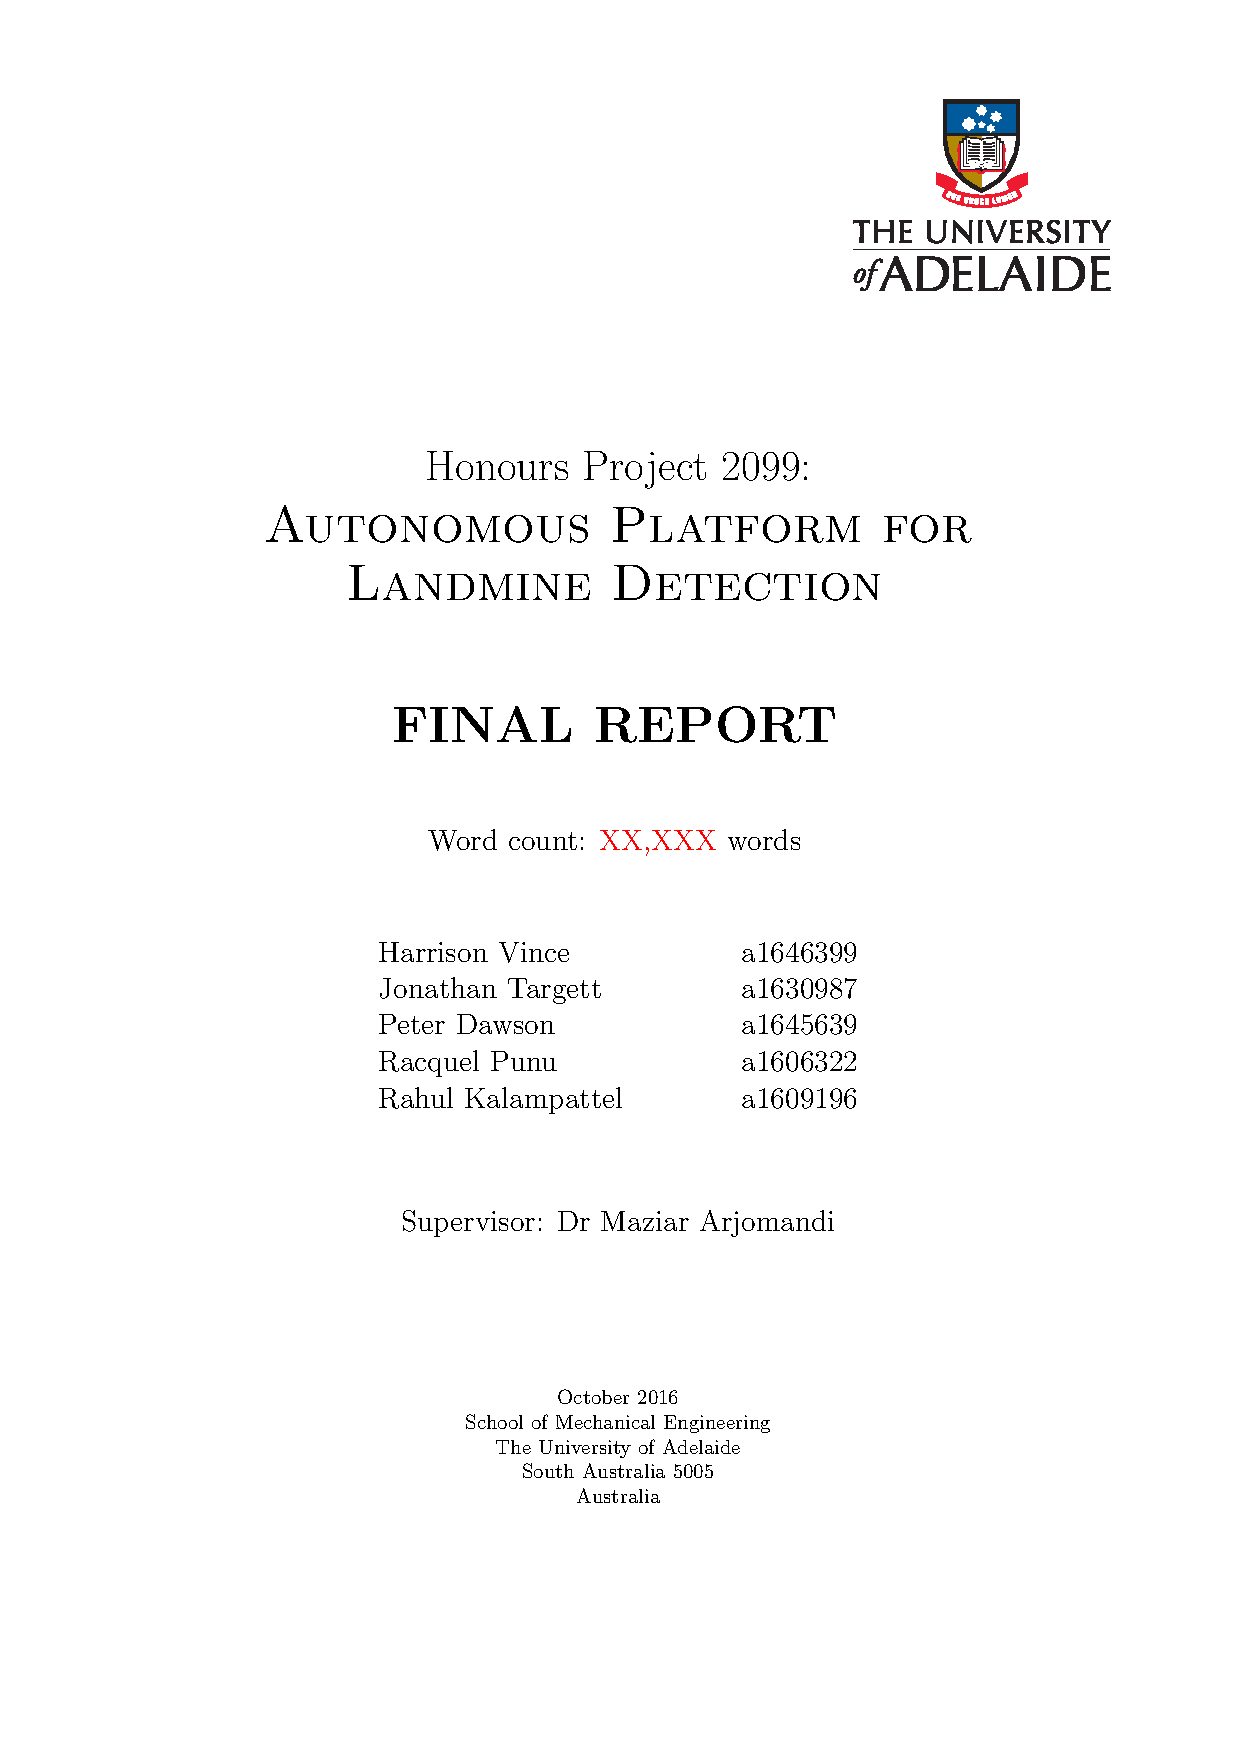
\includepdf{0-Preamble/coverpage.pdf}	% Get cover page (output from separate project)

\pagenumbering{roman}	% Numbering style for preamble
\phantomsection
\addcontentsline{toc}{chapter}{Executive Summary}	% Manually add ES to ToC
\chapter*{Executive Summary}
% MAZIAR: Need more details regarding intro, background and motivation, project objectives, method to achieve  objectives and work done (achievements)
This report details the preliminary design work and current progress for Honours Project 2099: Autonomous Platform for Landmine Detection. The Defence Science and Technology Group provided the primary motivation for the project, which was to reduce the risk to Australian Defence Force personnel who are tasked with demining activities. Therefore, the goal for this project is to develop and test an autonomous and unmanned multi-sensor system for landmine detection. 

A scenario of operations is presented, describing the basic system requirements for both the platform and sensor equipment. The resultant operating conditions are described as flat ground with dry, loose, sandy soil containing no vegetation or obstructions. Benchmarking and literature reviews were conducted on all necessary subsystems, primarily platform options, automation techniques, navigation and landmine detection methods. This highlighted the challenges associated with multi-sensor systems being able to identify a landmine from raw data and automation issues arising from waypoint navigation due to the limitations of path tracking. The challenges from the literature review of current landmine detection methods and autonomous platforms are used and expanded upon in the concept design. 

A DSTG supplied quad bike is chosen as our platform as it satisfied all predefined requirements, as well as having a pre-existing remote control system installed.

%as it has an existing remote control system, reducing project risk and development time. \textcolor{red}{this is the reason it was chosen over a tracked vehicle. it was mainly chosen because it satisfied all the requirements. Its probably fine but could also consider something like: ...chosen as our platform as it excelled in all platform requirements and also had an existing remote control system pre insta.......} \textcolor{blue}{A DSTG supplied quad bike is selected as the platform as it excelled in all platform requirements benchmarked against the project's primary objectives...... - (Should be after the primary objectives, which should be somewhere after the  }

Path tracking is to be conducted through the pure pursuit method which excels at path tracking for low driving speeds and discontinuous curvatures, which are expected to be traversed by the platform.
The platform automation will be conducted through with use of PID control to ensure accurate system control. Landmine detection will be provided via a set of scanning algorithms independently classifying detected objects, with a consensus on the probability of a detected object being a mine determined by a machine learning algorithm. 
The electronics required to integrate all systems and provide the control and necessary processing power are to be compromised of two main components: microcontrollers and desktop computing equipment. 
The microcontrollers are chosen to handle the low level input and output automation functions, while the desktop computing equipment will act as the central software location handling all the intensive computational processing. 
Various sensor mount designs are explored with the aim to provide minimal signal interference and maximise signal to noise ratios for the detection equipment. 
The final design will have the Ground Penetrating Radar closest to the platform while the metal detector will have a clearance of 500 mm from any metallic objects.
The mount will be constructed out of PVC and fibreglass to ensure no interference with the metal detector signal output.  

A more thorough design process for the chosen concept designs resulted in the detailed design. These designs will be used as the reference point for the construction and development of the whole system.  
Project management provides a high level overview of various management aspects of the project. The status update highlights that the project is behind schedule due to a change in the project scope to ensure funding. Delays in sponsorship signatures and equipment loan agreements have resulted in further delays but large amounts of work on software and signal processing has been completed. 
A reviewed Gantt chart and project breakdown structure are provided to take into consideration the delays to date. 
 
 Finally, the progress that has been made on the project to date is summarised, and an outline is given of how and when future work will be carried out. 

 

% This document is a proposal for Honours Project 2099: Autonomous Platform for Landmine Detection. The main objective of this project is to develop and test a multi-sensor system for landmine detection, to be mounted on a mobile platform; a secondary objective is to design a framework for the automation of this platform. It is intended that this project will serve as a technology demonstrator for the next generation of autonomous landmine detection systems. 

% The key stakeholders are introduced, with a description of the required roles for each individual. These include their high-level roles and responsibilities. 

% The primary project goals are then listed, these being the tasks which shall be completed in order for the project to be deemed a success. Extended goals are also suggested; these may be difficult or outside the scope of the project, but should be undertaken if time permits after the completion of the primary goals. Both of these are to be measured against the project specifications. The deliverables listed are those items which shall be produced over the course of the project, including reports and presentations, which demonstrate that progress has been made in achieving the goals. 

% The various hardware and software resources required for the completion of the project are outlined. A work breakdown of the project then follows, where these resources, as well as human resources, are assigned to various tasks. This information is also presented on a Gantt chart, which provides a timeline for the completion of the project. Together, these two items make up the research plan. 

% Finally, a preliminary estimate of the budget for the project is made. Based on this estimate, potential sponsorship in excess of \$X,XXX will be required in order for the project goals to be feasible.

\newpage
\phantomsection
\addcontentsline{toc}{chapter}{Disclaimer}	% Manually add ES to ToC
\chapter*{Disclaimer}
As the authors of this report, we declare that the material contained within is entirely our own work, unless otherwise specified. All work from other sources has been referenced accordingly. 
\vspace{0.4in}

% Update with correct images for signatures when ready, change dates as well

\noindent\begin{tabular}{ll}
\raisebox{-0.4in}[0pt][0pt]{
\includegraphics[height=0.7in]{0-Preamble/Rahul.jpg}}&\raisebox{-0.2in}{24/10/2016}\\
\makebox[2.5in]{\hrulefill} & \makebox[1.4in]{\hrulefill}\\
Harrison Vince & Date\\[0.4in]% adds space between the two sets of signatures
\raisebox{-0.4in}[0pt][0pt]{
\includegraphics[height=0.7in]{0-Preamble/Rahul.jpg}}&\raisebox{-0.2in}{24/10/2016}\\
\makebox[2.5in]{\hrulefill} & \makebox[1.4in]{\hrulefill}\\
Jonathan Targett & Date\\[0.4in]% adds space between the two sets of signatures
\raisebox{-0.4in}[0pt][0pt]{
\includegraphics[height=0.7in]{0-Preamble/Rahul.jpg}}&\raisebox{-0.2in}{24/10/2016}\\
\makebox[2.5in]{\hrulefill} & \makebox[1.4in]{\hrulefill}\\
Peter Dawson & Date\\[0.4in]% adds space between the two sets of signatures
\raisebox{-0.4in}[0pt][0pt]{
\includegraphics[height=0.7in]{0-Preamble/Rahul.jpg}}&\raisebox{-0.2in}{24/10/2016}\\
\makebox[2.5in]{\hrulefill} & \makebox[1.4in]{\hrulefill}\\
Racquel Punu & Date\\[0.4in]% adds space between the two sets of signatures
\raisebox{-0.4in}[0pt][0pt]{
\includegraphics[height=0.7in]{0-Preamble/Rahul.jpg}}&\raisebox{-0.2in}{24/10/2016}\\
\makebox[2.5in]{\hrulefill} & \makebox[1.4in]{\hrulefill}\\
Rahul Kalampattel & Date
\end{tabular}
\newpage

\phantomsection
\addcontentsline{toc}{chapter}{Acknowledgements}	% Manually add ToC to ToC
\chapter*{Acknowledgements} 
\textcolor{red}{Starting to list some people we could acknowledge.
\begin{enumerate}
\item Maziar Arjomandi
\item Workshop staff (Rob Dempster, can't think of anyone else you helped much)
\item Electronics workshop staff (Phil Schmidt)
\item DSTG people (Canicious Abeynayake)
\item Other (Marc Simpson)
\end{enumerate}}
\newpage

\phantomsection
\addcontentsline{toc}{chapter}{Contents}	% Manually add ToC to ToC
\renewcommand{\baselinestretch}{1.2}\normalsize 	% 1.2 line spacing
\tableofcontents
\renewcommand{\baselinestretch}{1.3}\normalsize 	% 1.3 line spacing
\newpage

\phantomsection
\addcontentsline{toc}{chapter}{List of Figures}	% Manually add LoF to ToC 
\listoffigures
\newpage

\phantomsection
\addcontentsline{toc}{chapter}{List of Tables}	% Manually add LoT to ToC
\listoftables
\newpage

% Uncomment the three lines below to split nomenclature into two columns
% \renewcommand*{\nompreamble}{\begin{multicols}{2}}
% \renewcommand*{\nompostamble}{\end{multicols}}
% \setlength{\columnsep}{3em}

\printnomenclature
\newpage

\end{document}